%%%%%%%%%%%%%%%%%%%%%%%%%%%%%%%%%%%%%%%%%%%%%%%%%%
\subsection{Why (sub)millimetre wavelength observations?}
%%%%%%%%%%%%%%%%%%%%%%%%%%%%%%%%%%%%%%%%%%%%%%%%%%



%%%%%%%%%%%%%%%%%%%%%%%%%%%%%%%%%%%%%%%%%%%%%%%%%%
\subsection{ALMA}
The Atacama Large Millimeter/submillimeter Array
(ALMA) is an international radio telescope located in the Atacama Desert in northern Chile \citep{Wotten}. It has 66 antennas working together as an interferometer, with multiple array configurations with baselines ranging from 15 meters to approximately 15 km \citep{Wotten}. ALMA has an observing wavelength range of 0.3 to 10 mm \citep{Wotten}, allowing it to probe thermal emission from dust in protostellar disks. 

\question{Add something that ALMA is high resolution and sensitity?}

 % \quoted{To accurately model the features and disentangle the various polarization mechanisms, multiwavelength observations at very high resolution and sensitivity are required \citep{Stephens_2019}}. 

 
%%%%%%%%%%%%%%%%%%%%%%%%%%%%%%%%%%%%%%%%%%%%%%%%%%




%%%%%%%%%%%%%%%%%%%%%%%%%%%%%%%%%%%%%%%%%%%%%%%%%%
\subsection{Polarization Quantities}

The electromagnetic waves that ALMA measures can \note{need to find a better way to say this} be defined in the four Stokes parameters: \SI represents the total intensity, \SQ and $U$ describe the linear polarization, and \SV describes the circular polarization \citep{Rybicki}. In this project we only consider linear polarization and Stokes $I$, $Q$ and $U$ (i.e. no circular polarization). \question{no circular polarization in disks?}

%%%%%%%%%%%%%%%%%%%%%%%%%%%%%%%%%%%%%%%%%%%%%%%%%%




%%%%%%%%%%%%%%%%%%%%%%%%%%%%%%%%%%%%%%%%%%%%%%%%%%
\subsection{Why Multi-wavelength observations are important}
\label{sec: intro_mw}


As mentioned in Chapter \ref{sec: intro_polarization_mechanisms}, the observed polarization morphology and inferred dominant polarization mechanism have been found to change with observing wavelength. However, the dominant polarization mechanism does not depend on wavelength alone. Different observing wavelengths are sensitive to different grain sizes and optical depths \citep{Testi}, which reveal different mechanisms. By comparing the polarization fraction and morphology at multiple wavelengths, it is possible to disentangle the polarization mechanisms and place stronger constraints on grain sizes compared to what could be achieves with observations at a single wavelength \citep{Harrison, Kataoka_2015}. 


\note{In the plot of Pw vs a max I refer to this for the importance of mw observations for grain size}
%%%%%%%%%%%%%%%%%%%%%%%%%%%%%%%%%%%%%%%%%%%%%%%%%%




\subsection{HL Tau}


\quoted{HL Tau's polarization spectrum is particularly interesting: the disk's polarization morphology transitions from a pattern consistent with scattering at $\sim$870 $\mu$m to an elliptical pattern at $\sim$3 mm, with an intermediate pattern at $\sim$1.3 mm (Stephens et al. 2017). Recently, Lin et al. (2022) and Lin et al. (2024) have demonstrated that HL Tau's polarization spectrum could be explained by polarization from thermal emission and the scattering of aligned grains, also demonstrating that the polarization seen at high resolution in HL Tau at 870 $\mu$m could be explained by the same mechanisms. At longer wavelengths, thermal polarization dominates because the low optical depth makes scattering inefficient. At shorter wavelengths, scattering polarization dominates because the high optical depth makes scattering events frequent and dichroic extinction decreases the contribution from thermal polarization (Lin et al. 2022).}  \citep{Harrison2024}

% ------------------------------------------------
\begin{figure*}[h]
  \centering
  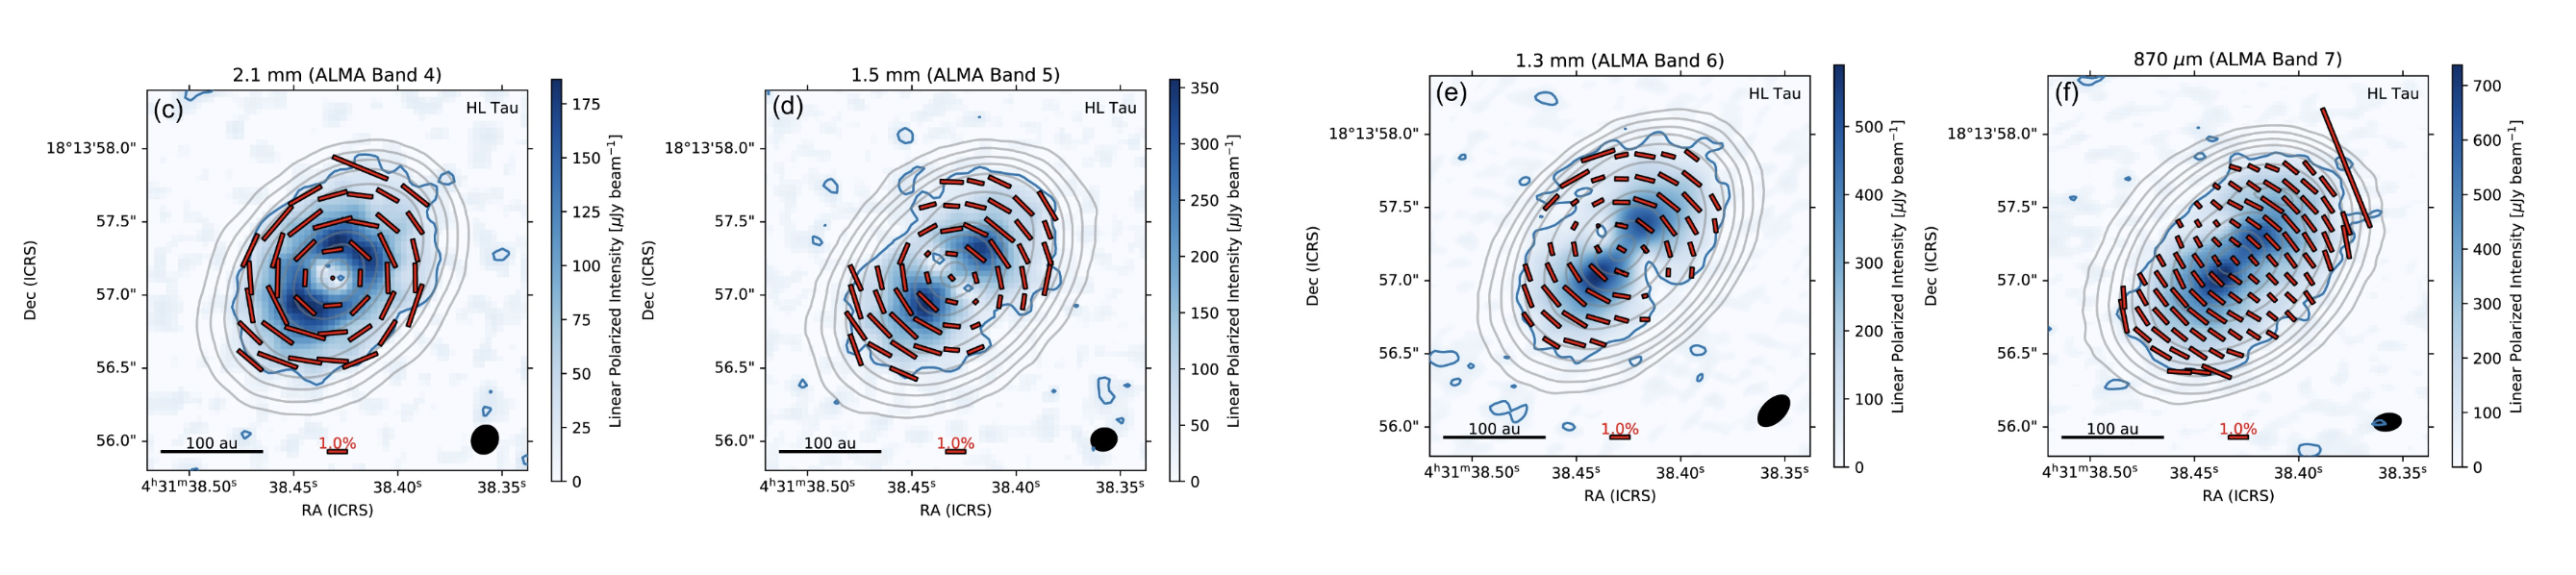
\includegraphics[width=1.1\textwidth]{../IMAGES/WRITEUP/NOTMINE/Lin2024Figure1.png}
  \caption{\add{caption} \note{Placeholder}}
  \label{fig: HLTauLin2024}
\end{figure*}
% ------------------------------------------------
